
\subsection*{1.}

\begin{center}
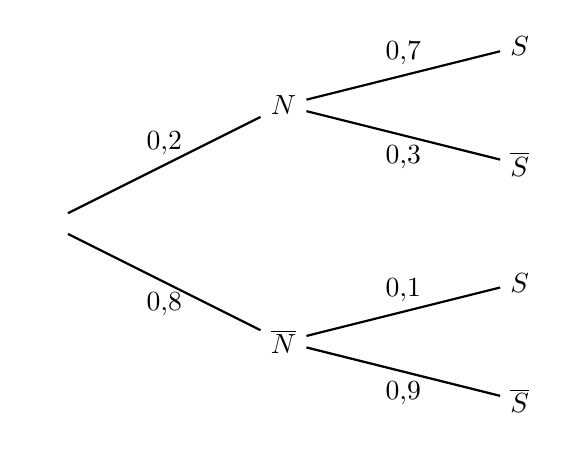
\begin{tikzpicture}[thick, scale=1.5] %{,}
\node (P_-1_0) at (-2,-1.5) {$\phantom{A}$};
\node (P_0_0) at (0,-0.5) {$N$};
\draw (P_-1_0) -- (P_0_0) node[midway, above] {$0{,}2$};
\node (P_1_0) at (2,-0) {$S$};
\draw (P_0_0) -- (P_1_0) node[midway, above] {$0{,}7$};
\node (P_1_1) at (2,-1) {$\overline{S}$};
\draw (P_0_0) -- (P_1_1) node[midway, below] {$0{,}3$};
\node (P_0_2) at (0,-2.5) {$\overline{N}$};
\draw (P_-1_0) -- (P_0_2) node[midway, below] {$0{,}8$};
\node (P_1_2) at (2,-2) {$S$};
\draw (P_0_2) -- (P_1_2) node[midway, above] {$0{,}1$};
\node (P_1_3) at (2,-3) {$\overline{S}$};
\draw (P_0_2) -- (P_1_3) node[midway, below] {$0{,}9$};
\end{tikzpicture}
\end{center}

\subsection*{2.}

Il faut calculer :
\[
p(N \cap S) = p(N) \times p_N(S) = 0{,}2 \times 0{,}7 = 0{,}14.
\]

\subsection*{3.}

On calcule :
\[
p(\overline{N} \cap S) = p(\overline{N}) \times p_{\overline{N}}(S) = 0{,}8 \times 0{,}1 = 0{,}08.
\]
D'après la loi des probabilités totales :
\[
p(S) = p(N \cap S) + p(\overline{N} \cap S) = 0{,}14 + 0{,}08 = 0{,}22.
\]

\subsection*{4.}

Soit :
\[
p_S(N) = \dfrac{p(S \cap N)}{p(S)} = \dfrac{p(N \cap S)}{p(S)} = \dfrac{0{,}14}{0{,}22} = \dfrac{7}{11} \approx 0{,}636.
\]

\subsection*{5.}

On a :
\[
p(N \cap \overline{S}) = 0{,}2 - 0{,}14 = 0{,}06 \quad \text{et} \quad p(\overline{N} \cap \overline{S}) = 0{,}8 - 0{,}08 = 0{,}72.
\]

On a donc le tableau suivant :

\[
\begin{array}{|c|c|c|c|c|}
\hline
\text{Événement} & N \cap S & N \cap \overline{S} & \overline{N} \cap S & \overline{N} \cap \overline{S} \\
\hline
\text{Dépense en €} & 70 & 45 & 25 & 0 \\
\hline
\text{Probabilité} & 0{,}14 & 0{,}06 & 0{,}08 & 0{,}72 \\
\hline
\end{array}
\]

On a donc :
\[
E(D) = 70 \times 0{,}14 + 45 \times 0{,}06 + 25 \times 0{,}08 + 0 \times 0{,}72 = 9{,}8 + 2{,}7 + 2 = 14{,}5 \, \text{(€)}.
\]
Sur un grand nombre de clients, la dépense moyenne par client est égale à \(14{,}50\) (€).

